\documentclass[10pt]{standalone}
\usepackage{commands}

\begin{document}
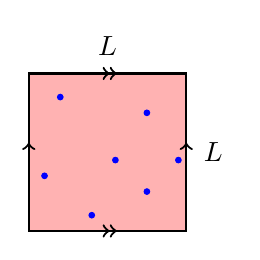
\begin{tikzpicture}[scale=1]
    \draw[black, thick, fill = white!70!red] (0, 0) -- (2, 0) -- (2, 2) -- (0, 2) -- cycle;
    \draw[fill=blue, draw=blue] (1.9, 0.9) circle (1pt);
    \draw[fill=blue, draw=blue] (1.5, 1.5) circle (1pt);
    \draw[fill=blue, draw=blue] (0.2, 0.7) circle (1pt);
    \draw[fill=blue, draw=blue] (0.8, 0.2) circle (1pt);
    \draw[fill=blue, draw=blue] (1.1, 0.9) circle (1pt);
    \draw[fill=blue, draw=blue] (0.4, 1.7) circle (1pt);
    \draw[fill=blue, draw=blue] (1.5, 0.5) circle (1pt);
    \node[above] at (1, 2.1) {$L$};
    \node[right] at (2.1, 1) {$L$};
    \draw[->, thick] (0, 0) -- (0, 1.12);
    \draw[->, thick] (2, 0) -- (2, 1.12);
    \draw[->>, thick] (0, 0) -- (1.12, 0);
    \draw[->>, thick] (0, 2) -- (1.12, 2);
\end{tikzpicture}
\end{document}